\section{Validation on Physical System}

The work in this section is still in development. I plan to test the ASMC on the system by having the assistie system act at different engagement levels. The tests will resemble the tests conducted on the simulated system discussed above. I will measure the position and applied torque to both the assistie and assistor systems and compare the measurements to a simulation of the same model.   


To test the controller,  a simple physical system was developed and built; this simplified system shows how the controller works on a real system.  \autoref{eq:armDyn} show the dynamics equation for a single-arm where $m$ is the mass of the arm and $l$ is the length of the arm. This system consists of two single degrees of arms; where one is the \textit{assistie} arm and the other is the \textit{assistor} arm.

\begin{equation}
    \tau = \frac{4}{3}ml^2 \ddot{\theta} + \frac{1}{2}ml \cos(\theta)
    \caption{Dynamics equation of a single arm of the system}
    \label{eq:armDyn}
\end{equation}

 The arms were connected with a Velcro strap piece of foam between the two arms to prevent the arms from bending inward. Each of the arms weighed approximately $90g$ and $0.3m$ long. An additional $20g$ was added to the \textit{assistie} arm to simulate the human system being heavier than the exoskeleton system. \autoref{fig:phyicalTestingSystem} shows the physical testing system. The arms are controlled by brushed DC motors with feedback from potentiometers for position sensing. A computer running Simulink acts as the high-level controller and a Teensy 4.0 \footnote{https://www.pjrc.com/store/teensy40.html} as the low-level controller communicating over a serial line. The motors are controlled by Performance Motion Digital motor controllers (Performance Motion Devices, Inc., 1 Technology Park Dr, Westford, MA 01886). Each of the motors is controlled by a 75W Atlas driver (MD211048/02VB) through the development board (MDK4LI0000V) (See Appendix C for the motor setup code) . The Teensy board communicates to the drivers over SPI by sending torque commands to each of the drivers, which delivers the proper current commands to the motors. \autoref{fig:phyicalTestingDiagram} shows the connection diagram; the computer is the high-level controller and the Teensy acts as the low-level controller. The controller was able to operate at $500Hz$. 
 



\begin{figure}[h!]
    \centering
    \includegraphics[width=\linewidth]{images/controllers/phyical system.png}
    \caption[Physical A-SMC Testing System]{Physical testing system of two connected arms. A Teensy 4.0 is used as a lower-level controller. Each arm has its own potentiometer and is controlled by a brushed DC motor. The arms are connected by a velcro strap and a piece of foam between the arms prevents the arms from bending inward. The DC motors are controlled by Atlas motor drivers. }
    \label{fig:phyicalTestingSystem}
\end{figure}


\begin{figure}
    \centering
    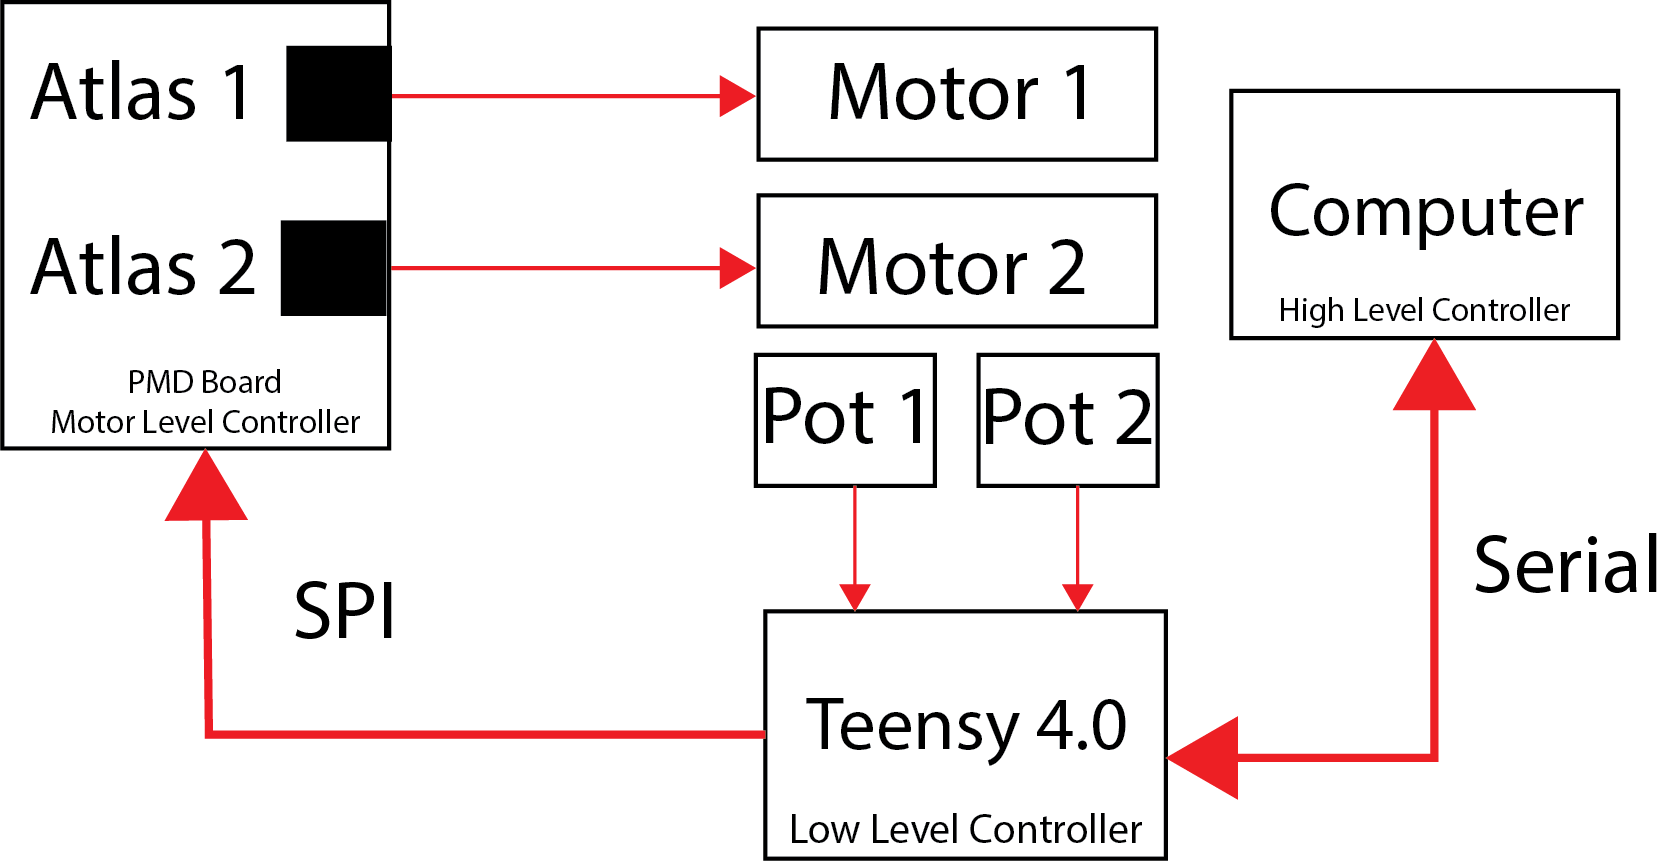
\includegraphics[width=\linewidth]{images/controllers/testing_system_diagam.png}
    \caption[Testing A-SMC System Diagram]{Connection diagram of the testing system. The computer communicates with the Teensy over serial protocol sending shown two torque command and receiving two position. The Teensy uses SPI to communicate with the motor drivers. }
    \label{fig:phyicalTestingDiagram}
\end{figure}


\autoref{fig:phyicalTraj} shows the comparison of the trajectories for both the \textit{assistie} and \textit{assistor} systems both a fully engagement and no engagement systems. The blue line is the desired motion, the red line is the path of the of the \textit{assistie} system with full engagement, the yellow line is the \textit{assistor} system with full engagement, the purple line is the path of the \textit{assistie} system with no engagement, and the green line is the path of the \textit{assistor} system with no engagement. 

The system was able to follow the desired motion when the system was the \textit{assistie} system was able to provide torque and when the A-SMC was fully engaged. \autoref{fig:phyicalTorque} shows the torque profiles for the systems, when the  \textit{assistie} torque was engaged the A-SMC controller was decreased. The blue line is the torque profile when the  \textit{assistie} system is full engaged and the orange line is when then \textit{assistie} system is not engaged. This result shows the the controller can be used on physicals systems. The paths of the  \textit{assistie} and  \textit{assistor} do not perfectly track each other, this is because of the soft connection between the two systems. A more rigid connection could solve this problem but may not accurately represent a real exoskeleton system. The The step like motion of the trajectories is caused by the low update speed and backlash in the motor gearboxes, by increase the control loop frequency a smooth control signal can be generated the will produce a better trajectory. The motors and gearboxes have a considerable about of backlash this causes in accuracy in the system positing and control. By increase and the control rate and using better gearboxes and motors this two problems should be mitigated.  This will also help the A-SMC controller which overshoot the final position of the desired motion slightly, a faster control rate will allow the controller to respond to the motion of the robot. 



\begin{figure}[h!]
    \centering
    \begin{subfigure}{\linewidth}
        \centering
        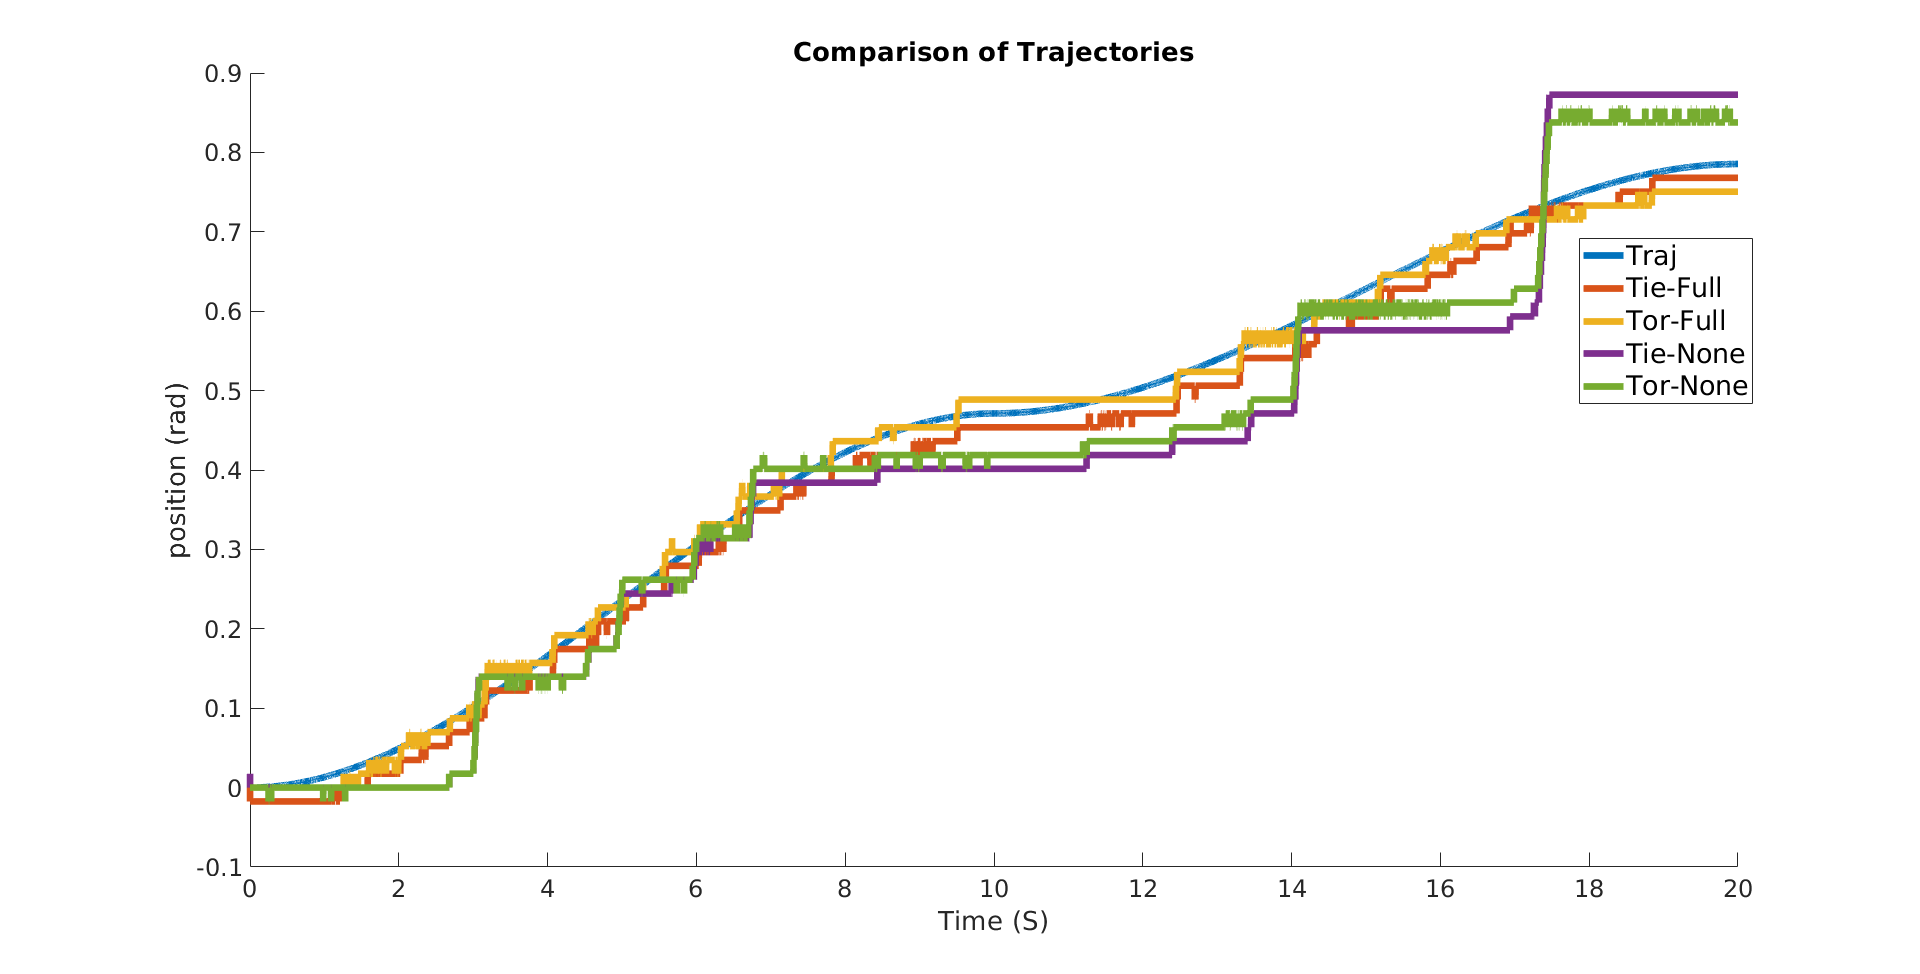
\includegraphics[width=\columnwidth]{images/controllers/comptraj2.png}
        \caption[Physical System Trajectory Tracking]{Comparison of a the trajectory on a physical system. The "None" systems have no engagement from the \textit{assistie} system. The "Full" systems has \textit{assistor} has fully engaged. }
        \label{fig:phyicalTraj}
    \end{subfigure}
        \begin{subfigure}{\linewidth}
        \centering
        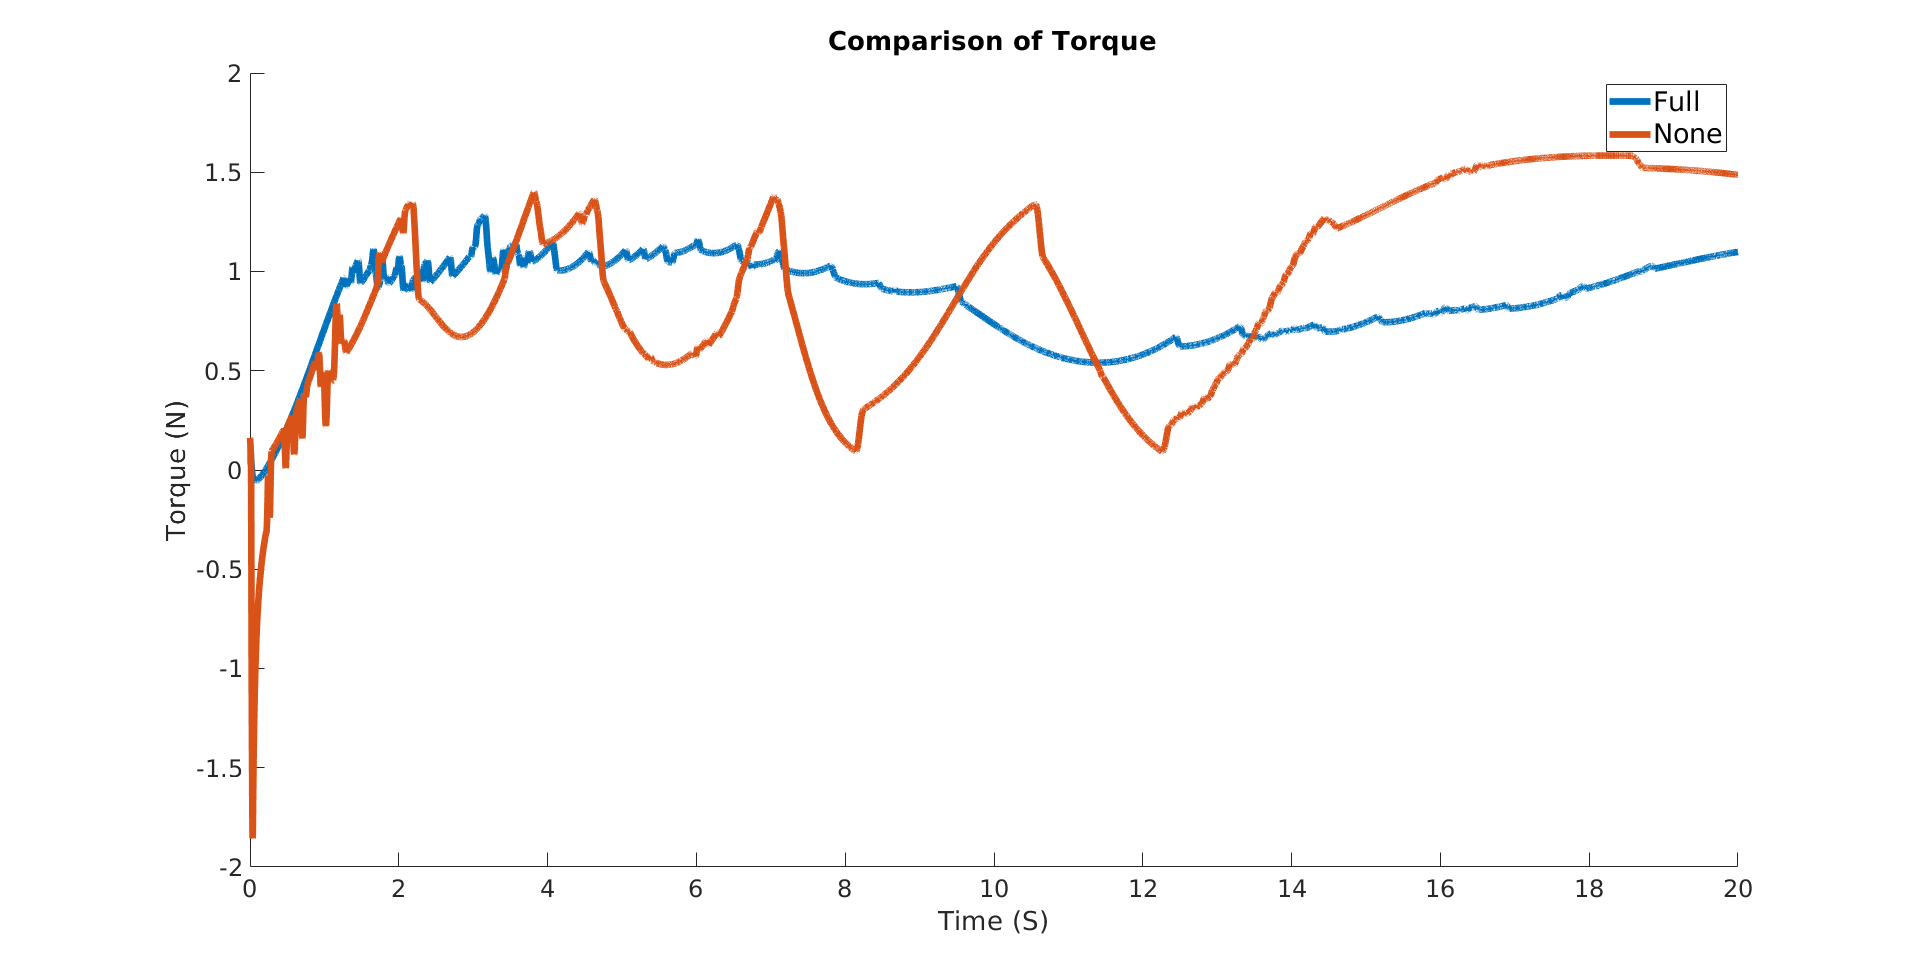
\includegraphics[width=\columnwidth]{images/controllers/comparisonOfTorque.png}
        \caption[Comparison of Torque for Full and No Engagement]{Comparison of a the torque on a physical system.}
        \label{fig:phyicalTorque}
    \end{subfigure}
    \caption[Physical System Engagement Levels]{Comparison of the torque profiles on the on the physical testing system.}
    \label{fig:phyicalSystemResults}
\end{figure}

 Application on real hardware comes with several challenges. Real systems must deal with sensor noise and communication speed, affecting how the controller responds to the model updates. This will improve the tracking error and smooth out the tracking signal displayed in both the  \textit{assistie}  and \textit{assistor} systems. These uncertainties need to be properly modeled to allow for offline tuning of the controller parameters. While the parameters for the physical system were tuned offline, they had the be slightly altered to handle the disturbance and friction in the system.  